% PDF version of the same figure (side by side, full width)
\begin{figure*}[t]
  \centering
  \begin{subfigure}[t]{0.45\textwidth}
    \centering
    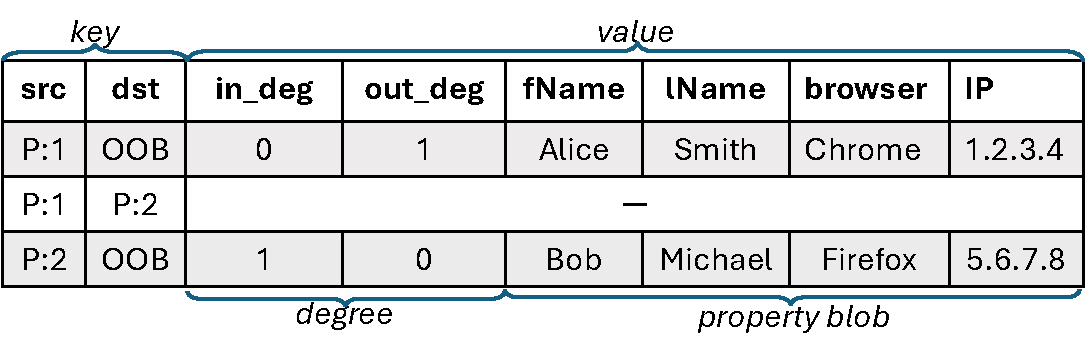
\includegraphics[width=0.85\textwidth]{content/fig/ekey_embedded_schema.pdf}
    \caption{Embedded properties: single edge\_out B-tree}
    \label{fig:schema:property:embedded}
  \end{subfigure}%
  \hfill
  \begin{subfigure}[t]{0.53\textwidth}
    \centering
    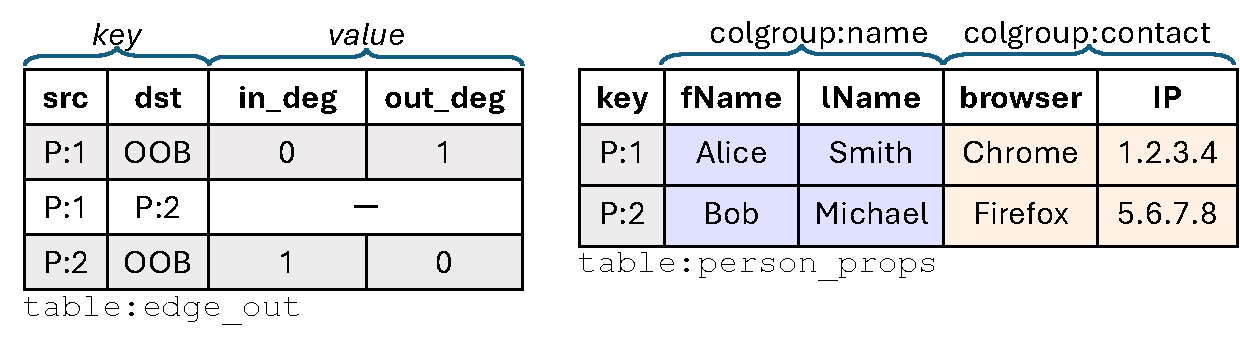
\includegraphics[width=0.85\textwidth]{content/fig/ekey_col_schema.pdf}
    \caption{Columnar properties: structural table + 2 property column groups }
    \label{fig:schema:property:columnar}
  \end{subfigure}
  \caption{Embedded vs.\ columnar property storage for Person vertices (EdgeKey).
    (a)~All properties packed into sentinel rows; every read fetches the full record.
    (b)~Sentinel rows store only degrees (8\,B); properties split into per-label column-group B-trees, so scanning one attribute reads only that group's pages.}
  \label{fig:schema:property}
\end{figure*}
